\chapter[A Teoria das Tranças]{A Teoria das Tranças}
\label{cap-3}
\chaptermark{}
%
\hfill%
\begin{minipage}{10cm}
\begin{flushright}
\rightskip=0.5cm
\textit{``Nature is written in mathematical language.''}
\\[0.1cm]
\rightskip=0.5cm
--- Galileu Galilei
\end{flushright}
\end{minipage}

\section{Introdução}
    %
    \begin{definition}[Trança (informal)]
    \label{def informal tranca}
    \index{Trança}
    	Uma \textbf{trança} de $n$ cordas nada mais é que um conjunto de $n$ cordas (que podem se cruzar ou não).
    	Contudo, em uma trança cada corda deve ``se mover'' monotonicamente da esquerda para a direita, isto é, 
    	se seguirmos qualquer corda da esquerda para a direita, ela não pode ``voltar'' (ir para a esquerda),
    	apenas ``ir'' (ir para a direita) e, também, duas cordas não podem passar uma por dentro da outra.
    \end{definition}
    %	
    \par\vspace{0.3cm} A Definição \ref{def informal tranca}, apesar de informal, ajuda a ter um entendimento
    intuitivo do conceito de trança. Essa definição será formalizada no Teorema \ref{apresentacao de B_n}.
    	
	\par\vspace{0.3cm} O conjunto das tranças de $n$ cordas (mais precisamente, o conjunto das classes 
	de equivalência das tranças de $n$ cordas) forma um grupo sob a operação de concatenação 
	(que será aqui tratada como produto), grupo esse denotado por $B_n$. 
	
	\par\vspace{0.3cm} Podemos ainda imaginar as tranças como cordas que tiveram suas extremidades coladas 
	em duas paredes opostas no espaço tridimensional. Nesse sentido, é fácil pensar em vários exemplos de tranças
	que surgem no cotidiano: a trança francesa no cabelo, os pães artesanais feitos com a massa trançada 
	(nas extremidades do pão as ``cordas'' da trança são ``coladas'' juntas, então o pão não é, em si, 
	uma trança, mas o padrão contido nele é). Veja os exemplos abaixo.
    %	
	\begin{figure}[H]
		\begin{center}
			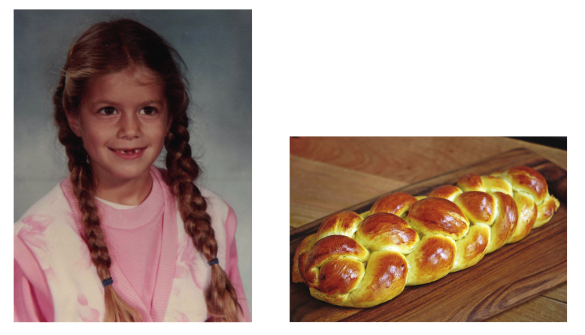
\includegraphics[width=6.1cm]{Images/exemplos_trancas.png}
		\end{center}
		\caption{Trança francesa (à esquerda) e pão trançado (à direita)}\label{exemplos de trancas}
	\end{figure}
    %
    \par\vspace{0.3cm} Podemos ainda representar as tranças através de diagramas, como mostram os exemplos abaixo.
    %
	\begin{figure}[H]
		\captionsetup{justification=centering}
		\begin{center}
			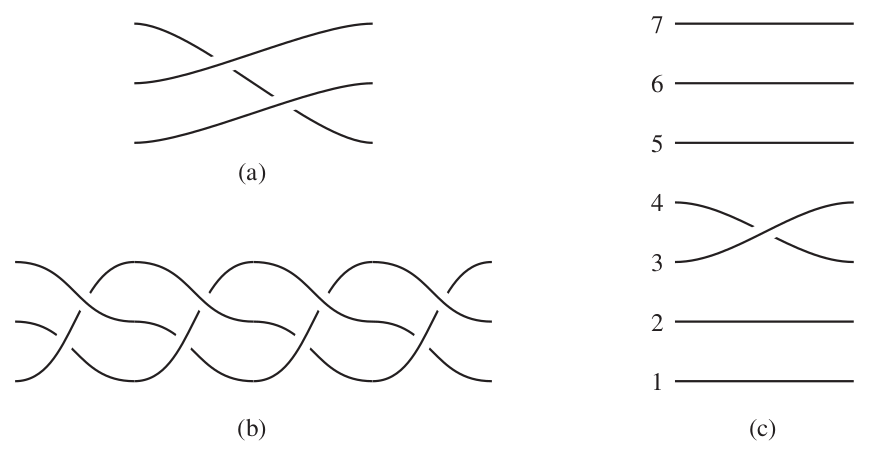
\includegraphics[width=12cm]{Images/exemplos_diagrama.png}
			\caption{
				(a) Uma trança de 3 cordas com 2 cruzamentos \\
				(b) A trança ``comum'' de 3 cordas (trança francesa) \\
				(c) Corda 3 passa sobre a corda 4}
				\label{diagramas de trancas}\end{center}
	\end{figure}
    %
	Note que cada corda recebe um número (a numeração pode ser feita de cima para baixo 
	ou de baixo para cima). Como dito anteriormente, podemos definir o produto de duas tranças como sendo 
	a concatenação dessas tranças. Além disso, também definimos a trança identidade de maneira bastante 
	intuitiva: ela é apenas o conjunto de $n$ cordas, sem nenhum cruzamento. Veja exemplos abaixo.
    %	
	\begin{figure}[H]
		\captionsetup{justification=centering}
		\begin{center}
			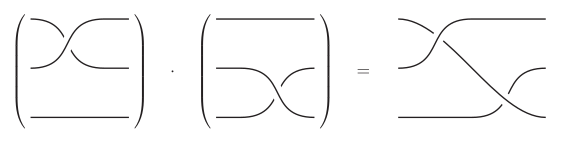
\includegraphics[width=12cm]{Images/produto.png}
		\end{center}\caption{O produto de duas tranças de 3 cordas
		}\label{produto de trancas}
	\end{figure}
    %	
	\begin{figure}[H]
		\captionsetup{justification=centering}
		\begin{center}
			
\includegraphics[width=5cm]{Images/identidade_b3.png}
		\end{center}\caption{A identidade em $B_3$}\label{identidade em b3}
	\end{figure}
    %
	\begin{figure}[H]
		\captionsetup{justification=centering}
		\begin{center}
			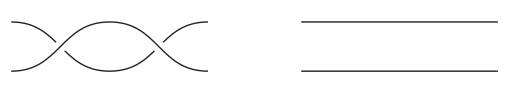
\includegraphics[width=10cm]{Images/identidade_b2.png}
		\end{center}\caption{Duas representações para a identidade em $B_2$. 
		Apesar de parecerem diferentes à primeira vista, elas pertencem à mesma classe de equivalência, 
		ou seja, são a mesma trança em $B_n$}\label{identidade b2}
	\end{figure}
	%
	Definido o produto da forma acima, o que significa ter o inverso de uma trança? 
	Por exemplo, qual seria o inverso da trança $\alpha$ na Figura \ref{diagramas de trancas}(b)?. 
	Bom, para saber isso devemos, primeiro, conhecer a identidade em $B_3$, que é mostrada acima.
	
	\par\vspace{0.3cm} Bom, como poderíamos estender $\alpha$ para fazê-la parecer a identidade? 
	É impossível: $\alpha$ tem cruzamentos, e desenhar mais coisas não vai mudar isso. Precisamos de uma 
	maneira de cancelar cruzamentos, de modo que as duas tranças na Figura \ref{identidade b2} 
	sejam equivalentes. 
	
	\par\vspace{0.3cm} Para isso, a ideia é que devemos ser capazes de mover as tranças do mesmo modo que 
	fazemos no espaço (ou seja, sem passar nenhuma corda por dentro de outra) e obter uma trança equivalente. 
	Para definir equivalência, é necessário dizer que quando movemos as tranças, as extremidades devem ficar 
	fixas (do contrário, qualquer trança seria equivalente à identidade).
	
	\par\vspace{0.3cm} Podemos ainda imaginar que as extremidades da esquerda de cada trança estão presas 
	à parede vertical $x=0$ no espaço tridimensional e as extremidades da direita estão presas à parede $x=1$.
	Nessa configuração, duas tranças são ditas \textit{equivalentes} se podemos mover uma delas, mantendo-a 
	entre as paredes e com as extremidades fixas, e fazê-la parecer a outra. 
	
	\par\vspace{0.3cm} Com essa definição, as duas últimas tranças da Figura \ref{identidade b2} 
	são equivalentes, assim como as tranças abaixo.
	%
	\begin{figure}[H]
		\captionsetup{justification=centering}
		\begin{center}
			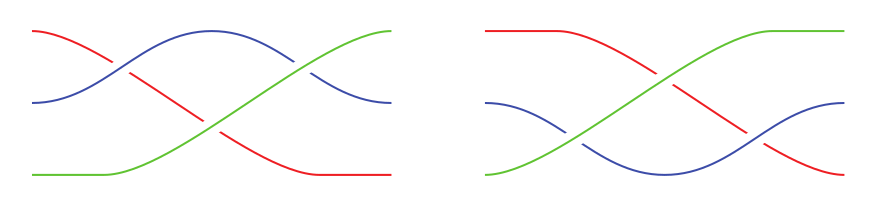
\includegraphics[width=12cm]{Images/fig_18_6.png}
		\end{center}\caption{Duas tranças equivalentes}\label{trancas equivalentes}
	\end{figure}   
	%
	Apenas um aspecto técnico: se fixarmos as paredes que limitam as tranças como 
	sendo $x = 0$ e $x=1$, devemos tomar mais cuidado com o que significa multiplicar duas tranças.
	Especificamente, para formar $\beta$ vezes $\beta'$, devemos transladar $\beta'$ uma unidade no eixo $x$, 
	tomar a união de $\beta$ com a versão transladada de $\beta'$ e redimensionar tudo por um fator de $1/2$. 
	Isso faz com que o produto de duas tranças seja também uma trança.
	
	\par\vspace{0.3cm} Desse modo, note que se fizermos o produto de uma trança $\gamma$ qualquer pela 
	segunda trança da Figura \ref{identidade b2}, seja à esquerda ou à direita, não alteraremos o número 
	de cruzamentos nem sua configuração, ou seja, não alteraremos a trança $\gamma$. Portanto, de fato, a 
	segunda trança da Figura \ref{identidade b2} é a identidade em $B_2$.
	
	\par\vspace{0.3cm} Note também que para obter o inverso de uma trança $\alpha$, basta espelharmos $\alpha$, 
	ou seja, o inverso de uma trança qualquer $\alpha$, denotado por $\alpha^{-1}$, nada mais é que a imagem
	espelhada de $\alpha$.
	%
	\begin{remark}
		Nesse sentido, encontrar o inverso de uma trança é parecido com encontrar o inverso de uma matriz: 
		devemos ir ``desfazendo'' a trança, de trás para frente (da direita para a esquerda), assim como o 
		inverso de um produto $ABC$ de matrizes é dado por $(ABC)^{-1} = C^{-1}B^{-1}A^{-1}$.
	\end{remark}
	%
	\begin{lemma}[Grupo de Tranças]
	\label{B_n grupo}
	\index{Grupo de Tranças}
		Para $n$ fixo, as (classes de equivalência de) tranças de $n$ cordas formam um grupo.
	\end{lemma}
	%
	\begin{proof}
		A identidade é evidente: ela é apenas o conjunto de $n$ cordas, sem nenhum cruzamento. 
		Anteriormente, enunciamos um procedimento para construir o inverso de uma trança 
		(inverso esse que também é uma trança), logo toda trança possui inverso. 
		A concatenação (que nada mais é que o produto) de duas 
		tranças de $n$ cordas nos dá outra trança também de $n$ cordas (como vimos anteriormente), 
		logo o conjunto é fechado para o produto. Por fim, a associatividade pode ser verificada através 
		de um diagrama, como o da Figura \ref{associatividade de trancas}.
		%
		\begin{figure}[H]
			\captionsetup{justification=centering}
			\begin{center}
				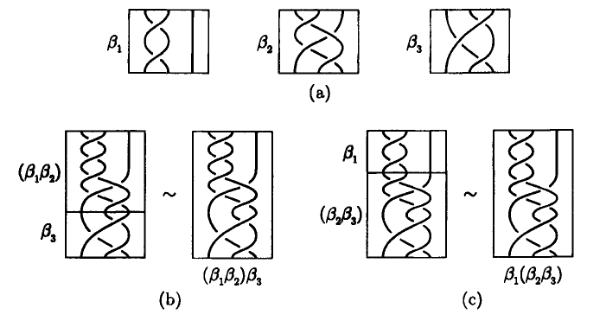
\includegraphics[width=7.1cm]{Images/associatividade.png}
			\end{center}\caption{Associatividade do produto de tranças}\label{associatividade de trancas}
		\end{figure}
		%
	\end{proof}
	%
	Quando estamos desenhando uma trança, podemos sempre usar a equivalência para 
	evitar que três ou mais cordas se cruzem no mesmo ponto do desenho. Também podemos fazer com que 
	nenhum cruzamento ocorra diretamente acima de outro, como mostra a figura abaixo.
	%
	\begin{figure}[H]
		\captionsetup{justification=centering}
		\begin{center}
			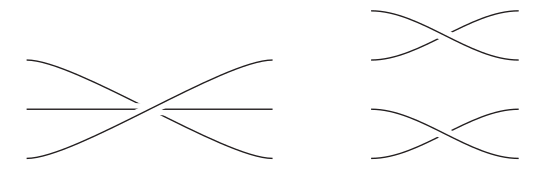
\includegraphics[width=12cm]{Images/desenhos_evitaveis.png}
		\end{center}\caption{Podemos evitar fazer desenhos como esses}\label{diagramas indesejaveis}
	\end{figure}
	%
	Por conta disso, podemos sempre ``cortar'' qualquer trança, usando linhas verticais, 
	de modo que cada pedaço seja uma trança que contenha somente um cruzamento, como abaixo.
	%
	\begin{figure}[H]
		\captionsetup{justification=centering}
		\begin{center}
			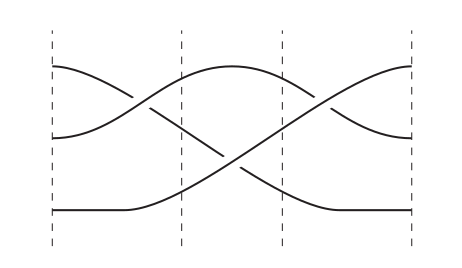
\includegraphics[width=8.6cm]{Images/fig_18_8.png}
		\end{center}\caption{Uma trança como produto de cruzamentos}\label{cortar trancas}
	\end{figure} 
	%
	Em outras palavras, $B_n$ é gerado pelo conjunto de todas as tranças de $n$ 
	cordas que têm exatamente um cruzamento. A trança em que a corda $i$ passa por cima da corda $i+1$ é 
	usualmente denotada por $\sigma_i$. Por exemplo, a Figura \ref{diagramas de trancas}(c) mostra a trança
	$\sigma_3$ em $B_7$. O seu inverso seria $\sigma_3^{-1}$, a corda 3 passando por baixo da corda 4. 
	Em geral, a trança em que a corda $i$ passa por baixo da corda $i+1$ (ou, equivalentemente, a corda 
	$i+1$ passa por cima da corda $i$) é denotada por $\sigma_i^{-1}$. 
	
	\par\vspace{0.3cm} Agora, podemos ver que $B_n$ é gerado pelo conjunto $\{ \sigma_1, \dots, \sigma_{n-1} \}$.
	Note, porém, que a notação $\sigma_i$ não diz em que grupo de trança estamos, exceto que deve ser pelo menos
	$B_{i+1}$. Por exemplo, o cruzamento $\sigma_2$ é um gerador de $B_3$, mas também de $B_4$, $B_5$ e assim por
	diante. O contexto geralmente deixa claro em qual grupo de tranças estamos. 
	
	\par\vspace{0.3cm} Tendo isso em mente, podemos escrever algumas das tranças vistas anteriormente em 
	termos dos geradores $\sigma_i$. Por exemplo, as tranças (a), (b) e (c) da 
	Figura \ref{diagramas de trancas} podem ser escritas, respectivamente, como $\sigma_2\sigma_1$,
	$(\sigma_1\sigma_2^{-1})^4$ e $\sigma_3$; a trança da Figura \ref{produto de trancas} pode ser 
	escrita como $\sigma_2\sigma_1^{-1}$; tanto a trança da Figura \ref{identidade em b3} quanto a trança 
	da Figura \ref{identidade b2} são a identidade em seus respectivos grupos ($B_3$ e $B_2$), podendo ser
	denotadas por $e$ ou, para evitar confusões, $1_3$ e $1_2$, respectivamente (de modo geral, podemos 
	denotar a identidade em $B_n$ por $1_n$); a trança da Figura \ref{trancas equivalentes} pode ser escrita 
	como $\sigma_1\sigma_2\sigma_1$ ou também como $\sigma_2\sigma_1\sigma_2$. Mais à frente veremos que esse 
	fato não é coincidência, mas uma relação muito importante para o grupo de trança.

	\par\vspace{0.3cm} Queremos agora pensar sobre como os diferentes $\sigma_i$ se relacionam. Note que 
	se $\sigma_i$ e $\sigma_j$ envolvem cordas completamente distintas, então eles comutam, como ilustrado abaixo.
	%
	\begin{figure}[H]
		\captionsetup{justification=centering}
		\begin{center}
			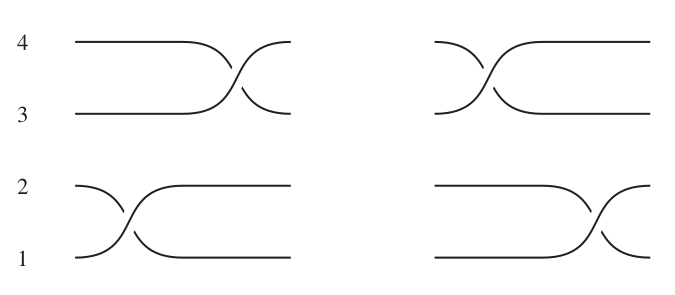
\includegraphics[width=10cm]{Images/comutatividade.png}
		\end{center}\caption{$\sigma_1\sigma_3$ e $\sigma_3\sigma_1$ são equivalentes.}
		\label{comutatividade de trancas}
	\end{figure}
	%
	\begin{remark}
		Intuitivamente, se dois cruzamentos envolvem cordas completamente distintas, então podemos 
		``deslizá-los'' livremente. Daí vem a comutatividade.
	\end{remark}
	%
	É natural pensar, então, que se dois cruzamentos têm uma corda em comum, 
	então a comutatividade não deve valer. De fato, isso é demonstrado pelo seguinte lema.
	%
	\begin{lemma}
	\label{vizinhos nao comutam}
		Dado $B_n$ e $\sigma_i$ um gerador de $B_n$, com $1\leq i\leq n-1$, os cruzamentos vizinhos não 
		comutam, isto é, $\sigma_i\sigma_{i+1}\neq\sigma_{i+1}\sigma_i$.
	\end{lemma}
	%
	\begin{proof}
		Basta fazer o desenho, como o do diagrama abaixo.
		%
		\begin{center}
			\begin{tikzpicture}
			\braid[braid colour=black,strands=3,braid start={(0,0)}]	{\sigma_1\sigma_2}
			\node[font=\Huge] at (4.5,-1.0) {\(\neq\)};
			\braid[strands=3,braid start={(5,0)}]
			{\sigma_2\sigma_1}
			\end{tikzpicture}
		\end{center}
		%
		Note que não é possível deslizar os cruzamentos de uma das tranças para obter 
		a outra e, consequentemente, cruzamentos vizinhos não comutam. 
	\end{proof}
	%
	Contudo, os $\sigma_i$'s vizinhos satisfazem a seguinte relação, 
	chamada \textit{relação de trança}:
	%
	\begin{equation*}
	    \sigma_i\sigma_{i+1}\sigma_i = \sigma_{i+1}\sigma_i\sigma_{i+1}.
	\end{equation*}
	%
	\begin{lemma}
		Em $B_n$, $\sigma_i\sigma_{i+1}\sigma_i = \sigma_{i+1}\sigma_i\sigma_{i+1}$, para todo $1\leq i\leq n-1$. 
	\end{lemma}
	%
	\begin{proof}
		Basta olhar o diagrama abaixo.
		%
		\begin{center}
			\begin{tikzpicture}
			\braid[braid colour=black,strands=3,braid start={(0,0)}]	{\sigma_1\sigma_2\sigma_1}
			\node[font=\Huge] at (4.5,-1.5) {\(=\)};
			\braid[strands=3,braid start={(5,0)}]
			{\sigma_2\sigma_1\sigma_2}
			\end{tikzpicture}
		\end{center}
		%
		Note que podemos obter o diagrama da direita a partir do diagrama da esquerda 
		da seguinte forma: a corda $i$ (à esquerda) é puxada um pouco para baixo; a corda $i+1$ (centro) 
		é puxada para a direita; e a corda $i+2$ (à direita) é puxada um pouco para cima.
		
		\par\vspace{0.3cm} Então, de fato $\sigma_i\sigma_{i+1}\sigma_i = \sigma_{i+1}\sigma_i\sigma_{i+1}$ 
		para todo $1\leq i\leq n-1$, como queríamos demonstrar.
	\end{proof}
	%
	Essas duas relações, a comutatividade e a relação de trança, implicam todas as 
	outras relações entre os $\sigma_i$. Em outras palavras:
	%
	\begin{theorem}
	\label{apresentacao de B_n}
		O grupo de trança tem a apresentação
		%
		\begin{equation*}
		    B_n 
		    = \langle \sigma_1, \dots, \sigma_{n-1} | \sigma_i\sigma_j 
		    = \sigma_j\sigma_i, \text{ para } |i - j|>1, \\ 
		    \sigma_i\sigma_{i+1}\sigma_i = \sigma_{i+1}\sigma_i\sigma_{i+1}, \text{ para } 1\leq i\leq n-2\rangle.
		\end{equation*}
		%
	\end{theorem}
	%
	Aceitaremos o Teorema \ref{apresentacao de B_n} sem demonstração.
	
	\par\vspace{0.3cm} As duas relações do Teorema \ref{apresentacao de B_n} nos ajudam a simplificar 
	e manipular palavras em $B_n$. Por exemplo, sabendo que $[a,b] = a^{-1}b^{-1}ab$, podemos manipular
	$(\sigma_i\sigma_{i+1})^{-1}[\sigma_{i+2}\sigma_i^{-1}, \sigma_i\sigma_{i+1}^{-1}]\sigma_i\sigma_{i+1}$ 
	para obter $\sigma_{i+2}\sigma_i^{-1}$ da seguinte forma:
	%
	\begin{align*}
	    &(\sigma_i\sigma_{i+1})^{-1}[\sigma_{i+2}\sigma_i^{-1}, \sigma_i\sigma_{i+1}^{-1}]\sigma_i\sigma_{i+1} \\
	    &= \sigma_{i+1}^{-1}\sigma_i^{-1}\sigma_i\sigma_{i+2}^{-1}\sigma_{i+1}\sigma_i^{-1}\sigma_{i+2}
	    \sigma_{i+1}^{-1}\sigma_i\sigma_{i+1}  \\
	    &= (\sigma_{i+1}^{-1}\sigma_{i+2}^{-1}\sigma_{i+1})\sigma_i^{-1}\sigma_{i+2}(\sigma_{i+1}^{-1}
	    \sigma_i\sigma_{i+1}).
	\end{align*}
	%
	Usando a relação de trança, deduzimos a seguinte relação:
	%
	\begin{align*}
	    \sigma_i^{-1}\sigma_{i+1}^{-1}\sigma_i = \sigma_{i+1}\sigma_i^{-1}\sigma_{i+1}^{-1} \\
	    \sigma_{i+1}^{-1}\sigma_i\sigma_{i+1} = \sigma_i\sigma_{i+1}\sigma_i^{-1}   
	\end{align*}
	%
	\par\vspace{0.3cm} Usando essa igualdade, temos
	%
	\begin{align*}
	    &(\sigma_{i+1}^{-1}\sigma_{i+2}^{-1}\sigma_{i+1})\sigma_i^{-1}\sigma_{i+2}(\sigma_{i+1}^{-1}
	    \sigma_i\sigma_{i+1}) \\
	    &= (\sigma_{i+2}\sigma_{i+1}^{-1}\sigma_{i+2}^{-1})\sigma_i^{-1}\sigma_{i+2}(\sigma_i\sigma_{i+1}
	    \sigma_i^{-1}) \\
    	&= \sigma_{i+2}\sigma_{i+1}^{-1}\sigma_{i+2}^{-1}\sigma_i^{-1}\sigma_i\sigma_{i+2}\sigma_{i+1}
    	\sigma_i^{-1} \\
    	&= \sigma_{i+2}\sigma_i^{-1}.
	\end{align*}
	%
	Outra aplicação do Teorema \ref{apresentacao de B_n} é o fato de que 
	$B_2\cong\mathbb{Z}$. Para perceber isso, basta notar que pelo Teorema \ref{apresentacao de B_n}, 
	$B_2 = \langle \sigma_1 | - \rangle$ e $\mathbb{Z}$ tem essa mesma apresentação. 
	
	\par\vspace{0.3cm} Também com o Teorema \ref{apresentacao de B_n}, podemos escrever 
	$B_3 = \langle \sigma_1,\sigma_2 \ | \ \sigma_1\sigma_2\sigma_1 = \sigma_2\sigma_1\sigma_2 \rangle$ e, 
	com isso, mostrar que $B_3 \cong\langle x,y \ | \ x^3=y^2 \rangle$ da seguinte maneira.
	
	\par\vspace{0.3cm} Da apresentação $B_3 = \langle \sigma_1,\sigma_2 \ | \ \sigma_1\sigma_2\sigma_1 
	= \sigma_2\sigma_1\sigma_2 \rangle$, podemos obter a relação equivalente 
	$(\sigma_1\sigma_2)^3 = (\sigma_2\sigma_1\sigma_2)^2 = (\sigma_1\sigma_2\sigma_1)^2$. Daí, usando 
	o Lema \ref{lema geradores}, sabemos que $\langle \sigma_1,\sigma_2 \rangle 
	= \langle \sigma_1\sigma_2,\sigma_2 \rangle = \langle \sigma_1\sigma_2, \sigma_2\sigma_1 \rangle 
	= \langle \sigma_1\sigma_2, \sigma_1\sigma_2\sigma_1 \rangle$. Portanto, fazendo 
	$x = \sigma_1\sigma_2$ e $y = \sigma_1\sigma_2\sigma_1$, concluímos que 
	$B_3 \cong \langle x,y \ | \ x^3=y^2 \rangle$.
	%
	\begin{remark}
		Um fato interessante é que como $SL(2,\mathbb{Z}) = \langle s,t \ | \ s^3 = t^2, t^4 = 1 \rangle$ 
		(não será demonstrado), e $B_3 = \langle x,y \ | \ x^3 = y^2 \rangle$, podemos ver que o conjunto de 
		relações de $B_3$ está contido no conjunto de relações de $SL(2,\mathbb{Z})$. Consequentemente, 
		pelo Teorema \ref{teorema de Dyck}, $SL(2,\mathbb{Z})$ é imagem homomórfica de $B_3$, i.e., 
		$B_3$ é homomorfo a $SL(2,\mathbb{Z})$. 
	\end{remark}
	%
	\begin{lemma}[Homomorfismo de comprimento]
	\label{homomorfismo de comprimento}
		Seja $l:B_n \to \Z$ tal que se $w$ é uma palavra nos geradores $\sigma_i$ e seus inversos, 
		então $l(w)$ é a soma dos expoentes 
		dos $\sigma_i$ em $w$. Então $l$ é um homomorfismo, chamado {\bf homomorfismo de comprimento}
		\index{Homomorfismo de comprimento}.
	\end{lemma}
	%
	\begin{proof}
		Sejam $w_1,w_2$ duas palavras em $B_n$ tais que $w_1=w_2$. Então, por definição, podemos, 
		após uma quantidade finita de inserções e remoções de elementos da forma $\sigma_i\sigma_i^{-1}$, 
		sair de $w_1$ e chegar em $w_2$. Como cada inserção/remoção desse tipo não altera a soma dos expoentes,
		pois estamos somando 0, então $l(w_1)=l(w_2)$, i.e., $l$ está bem definida. 
		
		\par\vspace{0.3cm} Agora, sejam $w_1,w_2$ duas palavras quaisquer em $B_n$. Note que $l(w_1w_2)$ é, 
		por definição, a soma dos expoentes de $w_1w_2$. Mas essa soma nada mais é do que a soma dos expoentes 
		de $w_1$ acrescida à soma dos expoentes de $w_2$, i.e., nada mais é do que $l(w_1)+l(w_2)$. Note que 
		essa igualdade vale ainda que o final de $w_1$ seja o inverso do início de $w_2$ (por exemplo, 
		$w_1 = \cdots\sigma_1\sigma_2^{-1}$ e $w_2 = \sigma_2\sigma_3\cdots$. Nesse caso, $l(w_1w_2)$ 
		continua sendo igual a $l(w_1) + l(w_2)$). Logo, $l(w_1w_2)=l(w_1)+l(w_2)$ e $l$ preserva a operação, 
		sendo portanto, homomorfismo.
		
		\par\vspace{0.3cm} Por fim, note também que $l$ é sobrejetora, uma vez que dado $n\in\mathbb{Z}$, 
		podemos tomar a palavra $w = \underbrace{\sigma_1\sigma_1\cdots\sigma_1}_{n}$ de forma a obter $l(w) = n$.
	\end{proof}
	%
	\begin{remark}
		A função $l$ do Lema \ref{homomorfismo de comprimento} é bem útil na verificação de equivalência 
		entre duas tranças. Isso porque a função $l$ é um invariante no grupo de tranças, i.e, se duas tranças 
		são equivalentes, suas imagens por $l$ (expoentes) devem ser iguais (segue da boa definição de $l$). 
		Daí, podemos usar a contra-positiva: se duas tranças têm expoentes diferentes, então elas não podem 
		ser equivalentes.
	\end{remark}
	%
	Da definição de $l$, é imediato que dada uma palavra $w$ qualquer, $l(w^{-1}) = -l(w)$.
	
	\par\vspace{0.3cm} Uma aplicação interessante de $l$ é a seguinte: se $\gamma$ é uma trança qualquer 
	conjugada ao seu inverso, i.e., se existe um trança $\delta$ tal que $\delta\gamma\delta^{-1} = \gamma^{-1}$,
	então $l(\gamma) = 0$.
	
	\par\vspace{0.3cm} De fato, se $\gamma$ é conjugada ao seu inverso, sabemos que $l(\delta\gamma\delta^{-1}) 
	= l(\gamma^{-1})$. Pela definição de $l$, temos que $l(\delta\gamma\delta^{-1}) = l(\gamma)$. Daí, 
	$l(\gamma) = l(\gamma^{-1}) = -l(\gamma)$ e, consequentemente, $l(\gamma) = 0$.
	
	\par\vspace{0.3cm} Podemos, ainda, pensar em tranças em termos de permutações, no sentido de que existe 
	uma correspondência $\pi: B_n\to S_n$ em que tomamos uma trança, ignorando se os cruzamentos são por cima ou por baixo, 
	e, numerando as posições inicial e final de cada corda, apenas lemos a permutação correspondente 
	(lembre que $S_n$ se refere ao grupo simétrico).
    %
	\begin{lemma}
	\label{B_n iso S_n}
		A função $\pi: B_n\to S_n$ definida anteriormente é um homomorfismo.
	\end{lemma}
	%
	\begin{proof}
		Seja $\psi:\underset{\sigma_i\mapsto(i\text{ }i+1)}{B_n\to S_n}$. Note que $\psi$ está bem definida, 
		uma vez que $\sigma_i=\sigma_j\Rightarrow\psi(\sigma_i)=\psi(\sigma_j)$. Sejam 
		$\sigma_i,\sigma_j\in B_n$ quaisquer. Suponha $|i-j|>1$. Então, 
		$\psi(\sigma_i\sigma_j)=(i\text{ } i+1)(j\text{ } j+1)=\psi(\sigma_i)\psi(\sigma_j)$. Se 
		$|i-j|=1$, podemos supor, sem perda de generalidade, que $j=i+1$. Então, temos
		$\psi(\sigma_i\sigma_{i+1})=(i\text{ } i+2\text{ } i+1)=(i\text{ } i+1)(i+1\text{ }
		i+2)=\psi(\sigma_i)\psi(\sigma_{i+1})$. Portanto, $\psi$ preserva a operação. 
		
		\par\vspace{0.3cm} Por fim, note também que $\psi$ é sobrejetora, uma vez que dada uma permutação 
		qualquer, sempre podemos construir uma trança cuja imagem por $\psi$ é tal permutação. Esse argumento 
		será formalizado mais adiante.
	\end{proof}
	%
	\begin{lemma}
	\label{apresentacao de S_n}
		Seja
		%
		\begin{align*} 
		G = 
		\langle \tau_1,\dots,\tau_{n-1} | &\tau_i\tau_j = \tau_j\tau_i, \text{ para }|i - j|>1,\\
		&\tau_i\tau_{i+1}\tau_i = \tau_{i+1}\tau_i\tau_{i+1}, \text{ para } 1\leq i\leq n-2, \\ 
		&\tau_i^2 = 1, \text{ para }1\leq i\leq n-1\rangle. 
		\end{align*}
		%
		Temos $S_n\cong G$, ou seja, 
		%
		\begin{align*} 
		S_n 
		= \langle \tau_1,\dots,\tau_{n-1} | &\tau_i\tau_j = \tau_j\tau_i, \text{ para }|i - j|>1,\\
		&\tau_i\tau_{i+1}\tau_i = \tau_{i+1}\tau_i\tau_{i+1}, \text{ para } 1\leq i\leq n-2, \\ 
		&\tau_i^2 = 1, \text{ para }1\leq i\leq n-1\rangle. 
		\end{align*}
		%
	\end{lemma}
	%
	\begin{proof}
		Primeiro, note que as transposições $\tau_i$ em $S_n$ satisfazem todas as relações de $G$. 
		Seja $\gamma:\underset{\tau_i\mapsto (i\text{ }i+1)}{G\to S_n}$. A boa definição de $\gamma$ e 
		a propriedade de preservar a operação são demonstradas de maneira análoga ao que foi feito no 
		Lema \ref{B_n iso S_n}.
		
		\par\vspace{0.3cm} Então, seja $(i\text{ }i+1)\in S_n$ qualquer e tome $\tau_i\in G$. Daí, 
		$\gamma(\tau_i) = (i\text{ }i+1)$ e, portanto, $\gamma$ é sobrejetora.
		
		\par\vspace{0.3cm} Por fim, suponha $\gamma(\tau_i) = \gamma(\tau_j)$. Então, $(i\text{ }i+1) 
		= (j\text{ }j+1)$, ou seja, $i = j$, o que é equivalente a $\tau_i = \tau_j$. Portanto, $\gamma$ é 
		injetora e, consequentemente, $\gamma$ é um isomorfismo de $G$ em $S_n$, como queríamos demonstrar.
	\end{proof}
	%
	Podemos, ainda, definir uma trança geometricamente, como a seguir.
	%
	\begin{definition}[Trança (geométrica)]
	\label{def geometrica tranca}
		Seja $I = [0,1]$. Uma trança geométrica em $n\geq 1$ cordas é um conjunto 
		$b\subset\mathbb{R}^2\times I$ formado por $n$ intervalos topológicos disjuntos chamados cordas 
		de $b$ tal que a projeção $\mathbb{R}^2\times I\to I$ mapeia cada corda homeomorficamente em $I$ e 
		%
		\begin{align*}
    		b\cap (\mathbb{R}^2\times \{ 0 \}) &= \left\{ (1,0,0), (2,0,0), \dots, (n,0,0) \right\}, \\
    		b\cap (\mathbb{R}^2\times \{ 1 \}) &= \left\{ (1,0,1), (2,0,1), \dots, (n,0,1) \right\}.
		\end{align*}
		%
	\end{definition}
	%
	Da Definição \ref{def geometrica tranca}, podemos ver que cada corda de $b$ 
	intercepta cada plano $\mathbb{R}^2\times\{t\}$, com $t\in I$, em exatamente um ponto. Também vemos 
	que cada corda de $b$ conecta um ponto $(i,0,0)$ a um ponto $(s(i), 0, 1)$, com $i,s(i)\in \{1, 2, \dots, n\}$.
	A sequência $(s(1), s(2), \dots, s(n))$ é uma permutação do conjunto $\{1, 2, \dots, n\}$ chamada permutação
	subjacente de $b$.
	%
	\begin{remark}
		Apesar de ser técnica, note que a Definição \ref{def geometrica tranca} nos diz algo simples; 
		o que ela está falando é que uma trança é um subconjunto $b$ da região $0\leq z\leq 1 $ 
		de $\mathbb{R}^3$. Além disso, as interseções entre $b$ e os planos $z = 0$ e $z = 1$ são, 
		respectivamente, o conjunto de pontos $\left\{  (1,0,0), \dots, (n,0,0)\right\}$ e o conjunto de 
		pontos $\left\{ (1,0,1), \dots, (n,0,1) \right\}$. Esses dois conjuntos são as extremidades de 
		cada corda da trança.
		
		\par\vspace{0.3cm} Note também que, da Definição \ref{def informal tranca}, sabemos que as 
		cordas de uma trança não podem passar uma por dentro da outra, ou seja, não podem se interceptar 
		e também sabemos que cada corda deve ir monotonicamente da esquerda para a direita, ou seja, não pode 
		haver loops. A Definição \ref{def geometrica tranca} respeita essas condições, uma vez que cada 
		plano $\mathbb{R}^2\times\{t\}$, com $t\in [0,1]$, intercepta cada corda de $b$ em exatamente um ponto,
		logo cada corda vai monotonicamente de cima para baixo, e as cordas de $b$ são disjuntas, isto é, 
		não se interceptam. Essa última propriedade significa que entre os planos $\mathbb{R}^2\times \{0\}$ 
		e $\mathbb{R}^2\times \{1\}$, o valor da coordenada $y$ varia: começa em $0$, aumenta (em módulo), 
		e retorna a $0$.
	\end{remark}
	%
	Podemos, ainda, reescrever a Definição \ref{def geometrica tranca} da seguinte forma:
	%
	\begin{definition}
	\label{outra def geometrica tranca}
		Seja $n\in\mathbb{N}$ fixo. Sejam ainda $n$ pontos distintos $p_1, \dots, p_n$ em $\mathbb{R}^2$. 
		Seja $(f_1, \dots, f_n)$ uma $n$-upla de funções $f_i:[0,1]\to\mathbb{R}^2$ tais que $f_i(0) = p_i$,
		$f_i(1) = p_j$ para algum $j=1,\dots,n$ e tais que os $n$ caminhos 
		%
		\begin{align*}
    		[0,1]&\to\mathbb{R}^2\times[0,1] \\
    		t&\mapsto (f_i(t), t)
		\end{align*}
		%
		chamados cordas, tenham imagens disjuntas. Essas $n$ cordas são chamadas de trança. 
		O grupo de trança $B_n$ em $n$ cordas é o grupo de classes de isotopia de tranças. O produto de uma 
		trança $( f_1(t), \dots, f_n(t) )$ por uma trança $( g_1(t), \dots, g_n(t) )$ é definido por
		%
		\begin{align}
		\label{def prod trancas}
    		(f\bullet g)_i(t) = 
    		\begin{cases}
        		f_i(2t), 0\leq t\leq \displaystyle{\frac{1}{2}} \\
        		g_j(2t-1), \displaystyle{\frac{1}{2}}\leq t\leq 1
    		\end{cases}\text{ sendo } j \text{ tal que }f_i(1) = p_j.
		\end{align}
		%
	\end{definition}
	%
	O interessante de se observar na Definição \ref{outra def geometrica tranca} é 
	o modo como o produto de tranças foi apresentado na Definição \ref{outra def geometrica tranca}. 
	O que a equação \ref{def prod trancas} nos diz é que para multiplicar a trança 
	$\alpha = ( f_1(t), \dots, f_n(t) )$ pela trança $\beta = ( g_1(t), \dots, g_n(t) )$, devemos 
	diminuir o ``tamanho'' de ambas as tranças pela metade e, em seguida, conectá-las, colocando $\alpha$ 
	``em cima'' de $\beta$. Outra maneira equivalente de pensar é que apenas ``encurtamos'' $\alpha$ por 
	um fator de $1/2$, sem transladá-la, e ``encurtamos'' $\beta$ também por um fator de $1/2$, mas 
	transladamos $1/2$ na direção negativa do eixo $\mathcal{O}z$. Essa definição é a mesma que a 
	Definição \ref{def informal tranca}, apenas formalizada!